%MARCOS RIAL DOCAMPO
%Presentación en diapositivas del TFG

\documentclass[12pt]{beamer}
\usetheme{Madrid}
\usecolortheme{dolphin}
\useoutertheme{smoothbars}
\useinnertheme{circles}
\setbeamercovered{invisible}
\setbeamertemplate{navigation symbols}{}

\usepackage[utf8]{inputenc}
\usepackage[spanish]{babel}
\usepackage{helvet}
\usepackage{amsmath}
\usepackage{amsfonts}
\usepackage{amssymb}
\usepackage{latexsym}
\usepackage{graphicx}
\usepackage{hyperref}
\usepackage{url}
\usepackage{epstopdf}
%\usepackage{natbib}
\usepackage{booktabs}
\usepackage{caption}

\author[Marcos Rial Docampo]{Marcos Rial Docampo\\
	\footnotesize{Tutores:\\Eduardo Corbelle Rico y Rafael Enrique Corrales Andino}}
\title[Análisis de Separabilidad Espectral]{\large{Análisis de separabilidad espectral de especies\\de mangle en el Golfo de Fonseca}}
\subtitle{Aplicación a la clasificación de imágenes Landsat}

\institute[USC-EPS]{Trabajo Fin de Grado \\Grado en Ingeniería en Geomática y Topografía\\Escuela Politécnica Superior de Lugo} 
\date{23 de febrero de 2016}
%\subject{}

\begin{document}

\begin{frame}[plain]
\begin{center}
	\includegraphics[scale=0.5]{./Imagenes/logo_ux.eps}
\end{center}
\maketitle
\end{frame}

\section{Introducción}
\subsection{Marco Global}
\begin{frame}
\only<1>{\includegraphics[width=\linewidth]{./Imagenes/Mangle2.jpg}}
\end{frame}

\begin{frame}
\begin{block}{}
	\begin{itemize}
		\item Sistema medioambiental extenso y complejo \pause
		\item Situado en zona intermareal de zonas tropicales y subtropicales \pause
		\item Compuesto por más de 80 especies forestales y 2000 animales \pause
		\item Dependiente de procesos externos \pause
		\item Ecosistema gravemente amenazado
	\end{itemize}
\end{block}
\end{frame}

\subsection{Objetivos}
\begin{frame}
\begin{block}{Objetivos generales}
	\begin{enumerate}[<+->]
		\item Evaluar la posibilidad de emplear imágenes multiespectrales de satélite para diferenciar distintas especies de mangle del Golfo de Fonseca.
		\item La respuesta espectral de las diferentes especies es lo suficientemente diferente como para permitir la clasificación de estas imágenes.
	\end{enumerate}
\end{block}
\end{frame}

\begin{frame}
	\begin{block}{Objetivos específicos}
		\begin{enumerate}
			\item<1-> Análisis de separabilidad espectral de las especies:
				\begin{itemize}
					\item \textit{Rhizophora mangle} o mangle rojo
					\item \textit{Laguncularia racemosa} o mangle blanco
					\item \textit{Avicennia germinans} o mangle prieto
				\end{itemize}
			\item<2-> Realizar una clasificación de imágenes de Landsat 8\\
			\item<3-> Estudiar el empleo de software libre
		\end{enumerate}
	\end{block}
\end{frame}

\subsection{Zona de estudio}
\begin{frame}
\only<1>{\includegraphics[width=\linewidth]{./Imagenes/localizacion.eps}}
\only<2>{\includegraphics[width=\linewidth]{./Imagenes/localizacion_elev.eps}}
\end{frame}

\section{Material y Métodos}
\subsection{Software}
\begin{frame}
	\begin{columns}
		\begin{column}{3.5cm} \vspace*{0.2cm}
			\begin{block}{}
				\begin{itemize}[<+->]
					\item R
					\item GRASS GIS QGIS
					\item \LaTeX
					\item JabRef, SmartGit
				\end{itemize}
			\end{block}
		\end{column}
		\begin{column}{7cm}
			\begin{block}{}
			\only<4> {\small	\url{https://github.com/MarcosRial/TFG}}
			\end{block}
		\end{column}
	\end{columns}
\end{frame}

\subsection{Técnicas de análisis espectral}
\begin{frame}
	\begin{columns}
		\begin{column}{5cm} \vspace*{0.5cm}
			\begin{block}{}
				\begin{enumerate}[<+- | alert@+>]
					\item Índice de Acuerdo Espectral
					\item Ángulo espectral
					\item Continuum Removal
				\end{enumerate}
			\end{block}
		\end{column}
		\begin{column}{5.5cm}
			\only<1>{$ IAE = \frac{\displaystyle\sum_{k=1}^m(CB_{i,k} - CB_{j,k})^{2}}{m} $}
			\only<2>{$\theta = arcos \frac{\displaystyle\sum_{k=1}^{m} \rho_{i,k} \rho_{j,k}}{\sqrt{\displaystyle\sum_{k=1}^{m} \rho_{i,k}^{2}} \sqrt{\displaystyle\sum_{k=1}^{m} \rho_{j,k}^{2}}}$}
			\only<3>{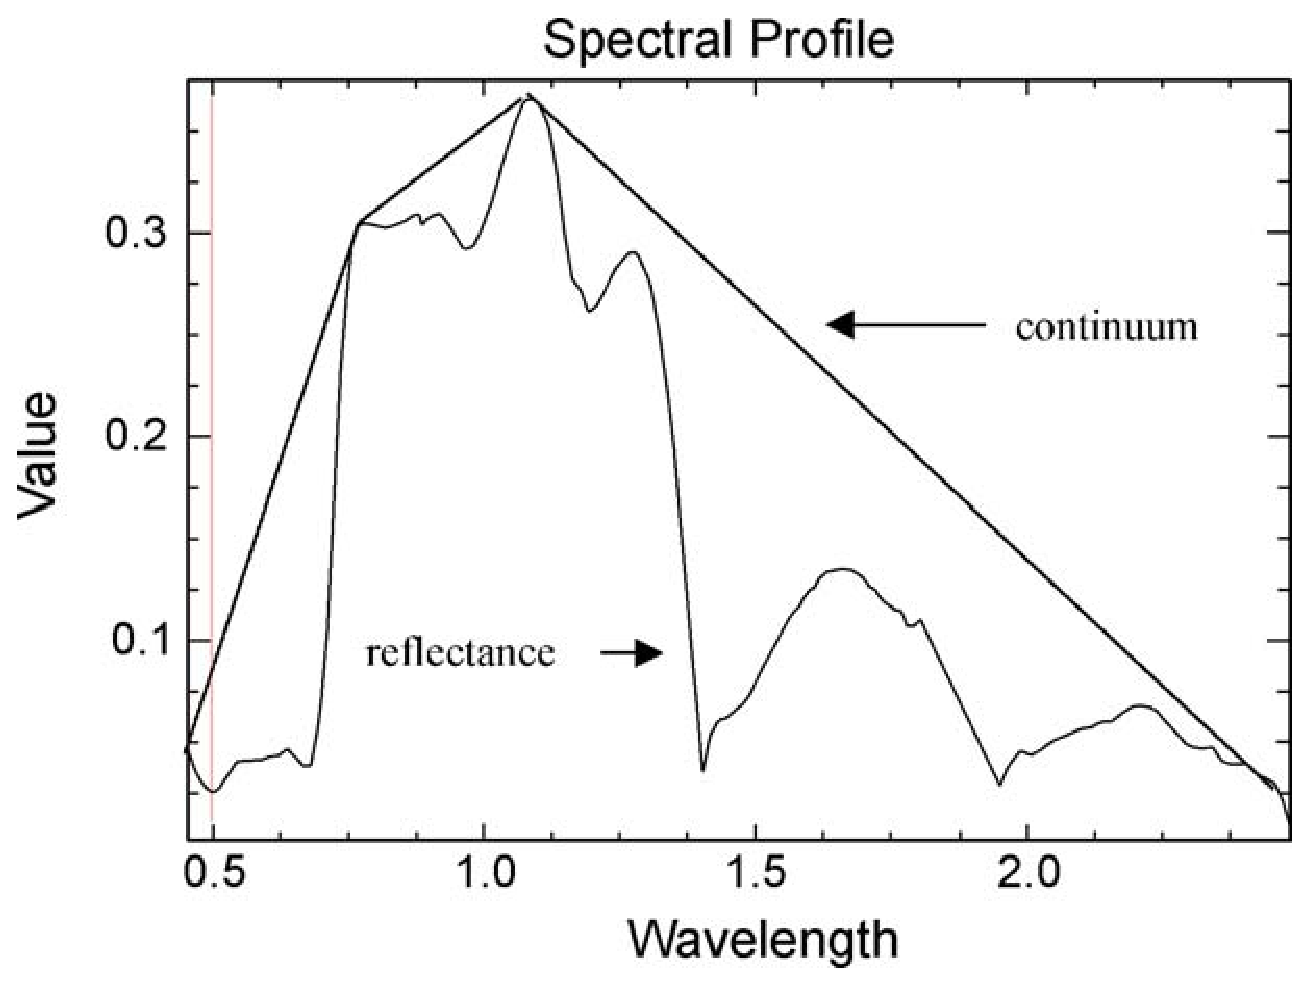
\includegraphics[width=0.9\linewidth]{./Imagenes/CR1.eps}}\\
			\only<3>{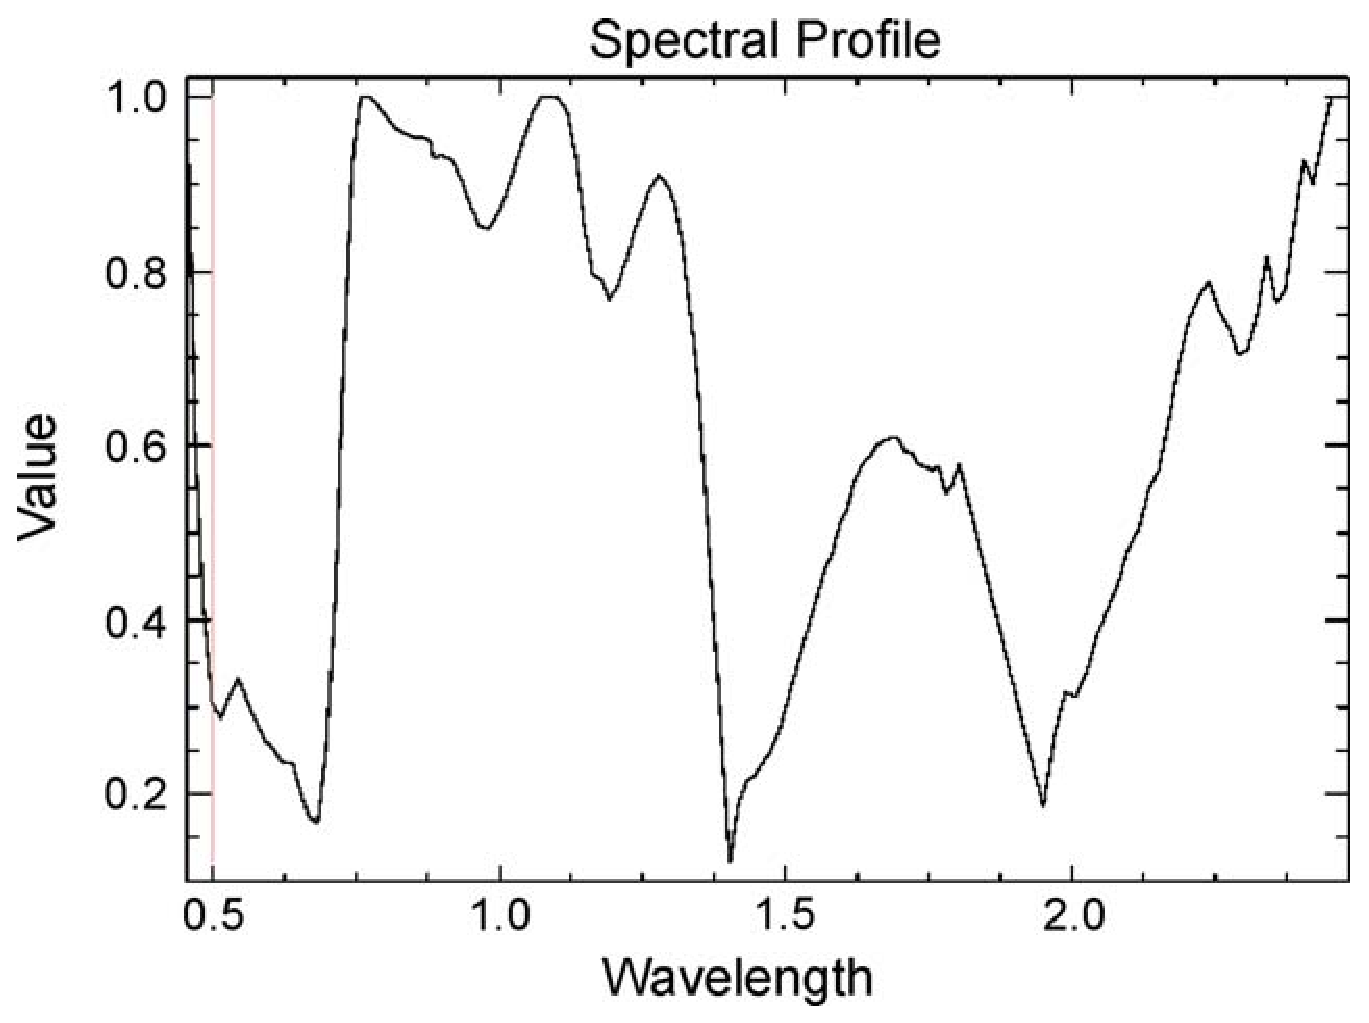
\includegraphics[width=0.9\linewidth]{./Imagenes/CR2.eps}}
		\end{column}
	\end{columns}
\end{frame}

\subsection{Imágenes Landsat}
\begin{frame}
	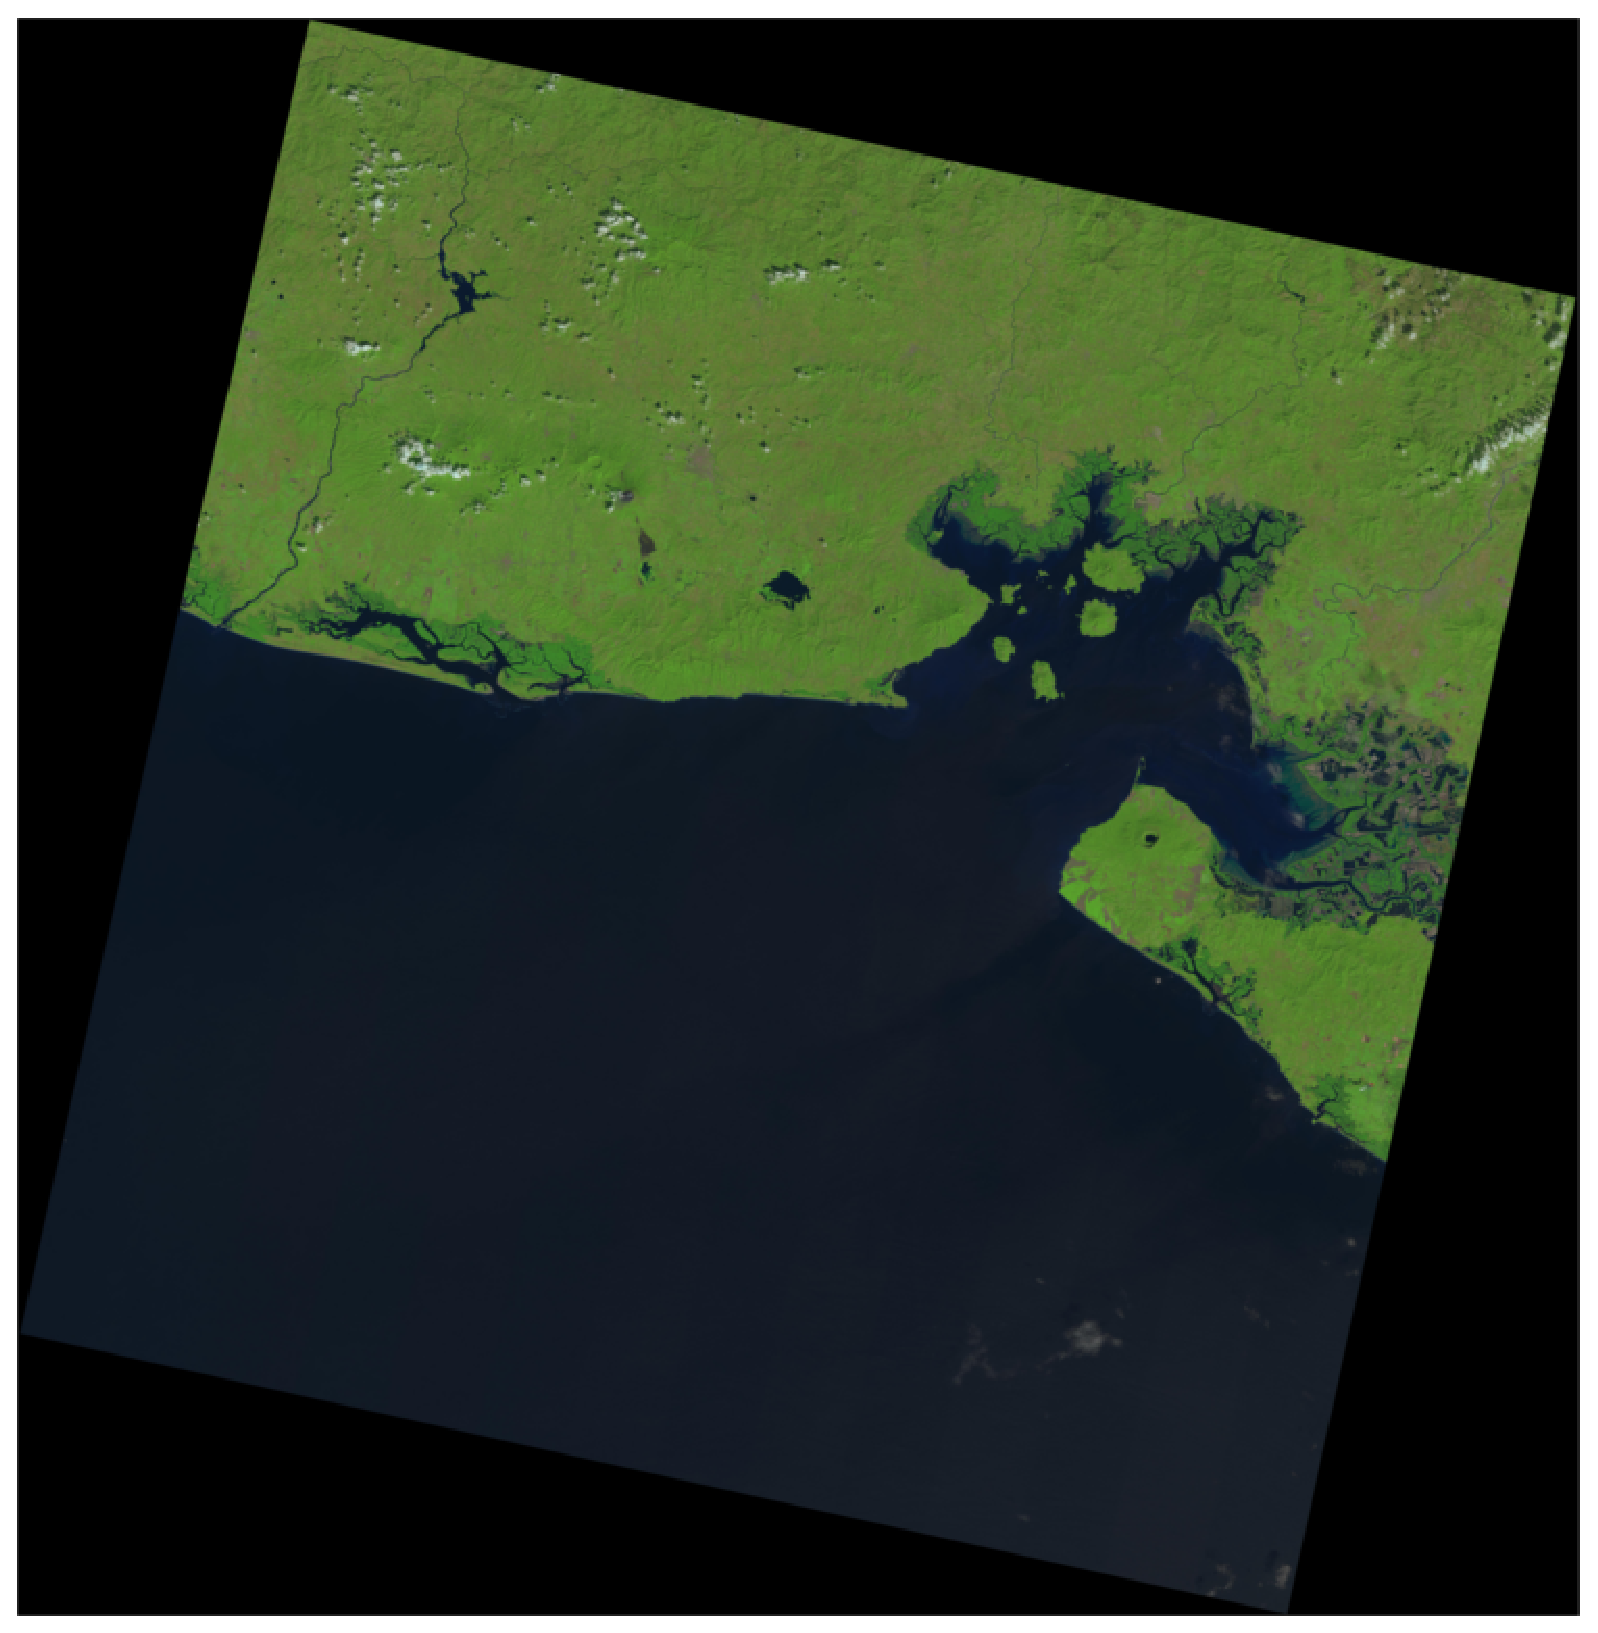
\includegraphics[width=0.5\linewidth]{./Imagenes/Landsat18.eps}
	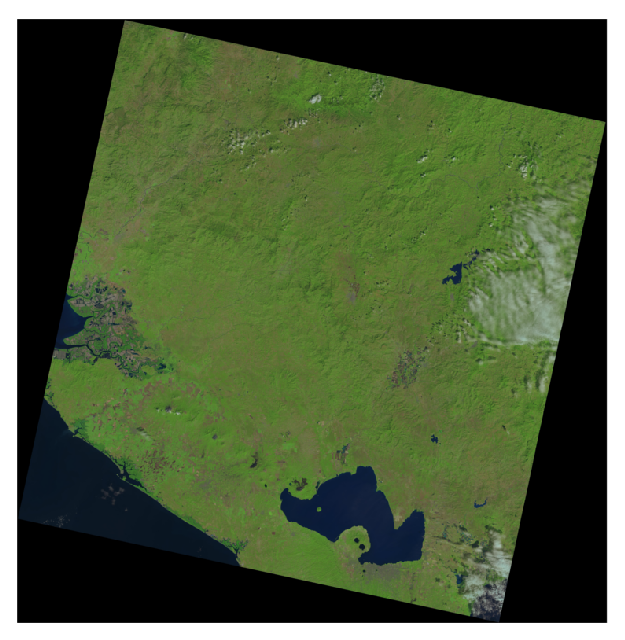
\includegraphics[width=0.5\linewidth]{./Imagenes/Landsat17.eps}\\
	{\color{red}{\scriptsize Landsat SR}}
	{\tiny \begin{table}
		\centering
		\begin{tabular}{@{}cccccccc@{}}
			\toprule[0.4mm]
			Imagen & Path & Row & Fecha & West & East & North & South \\
			\midrule
			1 & 18 & 51 & 23/11/2014 & -89.105062 & -86.987819 & 14.067713 & 11.946409 \\
			2 & 17 & 51 & 19/12/2014 & -87.549399 & -85.443030 & 14.062287 & 11.952632 \\
			\bottomrule[0.4mm]
		\end{tabular}
	\end{table}}
\end{frame}

\begin{frame}
	\begin{block}{Tratamientos a las imágenes}
		\begin{itemize}[<+->]
			\item Valores nulos de las imágenes
			\item Creación del mosaico
			\item Recorte de la imagen
			\item Filtro de paso bajo
		\end{itemize}
	\end{block}
\end{frame}

\subsection{Estudio Radiométrico}
\begin{frame}
	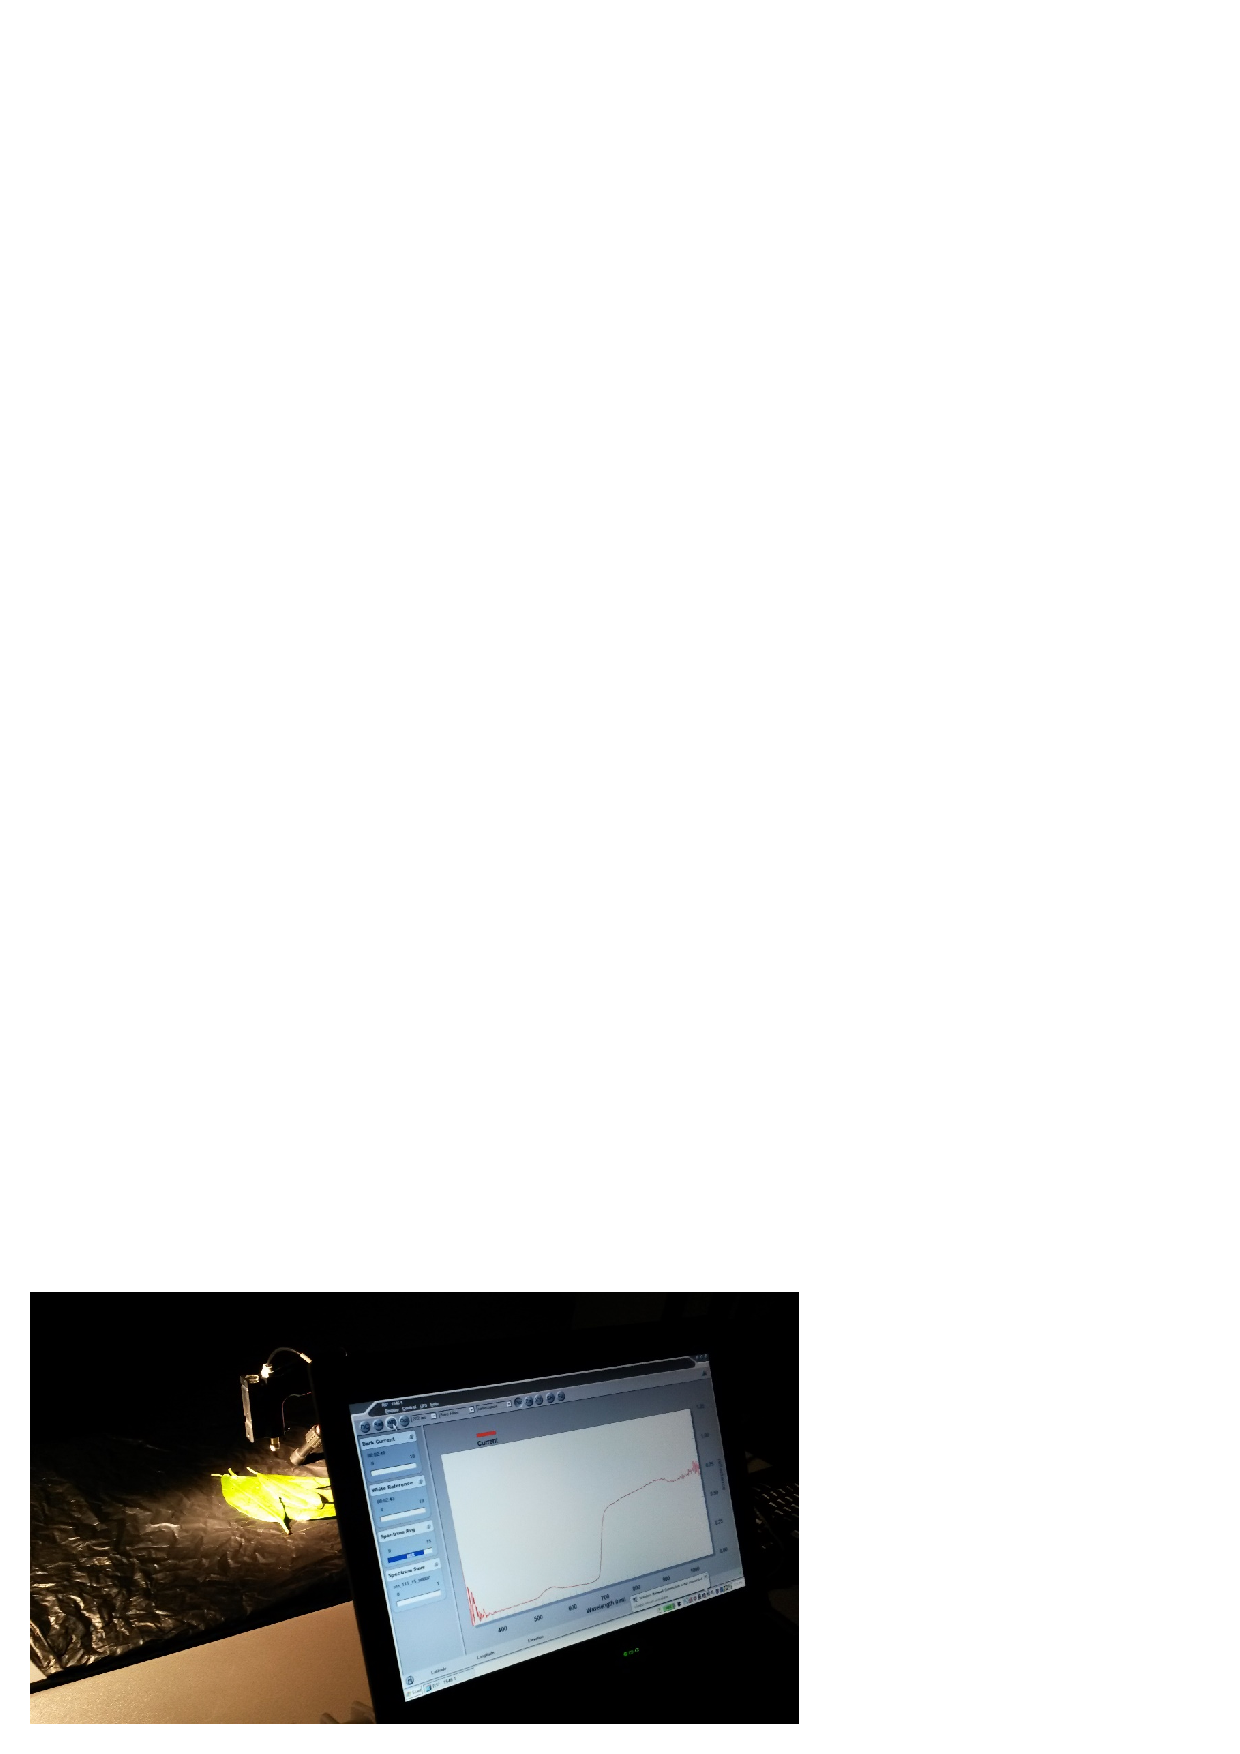
\includegraphics[width=\linewidth]{./Imagenes/Curva_espectral.jpg}
\end{frame}

\section{Resultados}
\subsection{Análisis de Separabilidad}
\begin{frame}
	\only<1>{\includegraphics[width=\linewidth]{./Graficos/1.png}}
	\only<2>{\includegraphics[width=\linewidth]{./Graficos/2.png}}
	\only<3>{\includegraphics[width=\linewidth]{./Graficos/3.png}}
	\only<4>{\includegraphics[width=\linewidth]{./Graficos/4.png}}
	\only<5>{\includegraphics[width=\linewidth]{./Graficos/5.png}}
	\only<6>{\includegraphics[width=\linewidth]{./Graficos/6.png}}
\end{frame}

\subsection{Índice de Acuerdo Espectral}
\begin{frame}
	\begin{table}
		\centering
\textit{{\footnotesize Valores de IAE para cada combinación de especies de mangle.}}\\
		\begin{tabular}{@{}cccc@{}}
			\toprule[0.4mm]
			& \textit{R. mangle} & \textit{L. racemosa} & \textit{A. germinans} \\
			\textit{R. mangle} & --- & 0,0083 & 0,0062 \\
			\textit{L. racemosa} & 0,0083 & --- & 0,0021 \\
			\textit{A. germinans} & 0,0062 & 0,0021 & --- \\
			\bottomrule[0.4mm]
		\end{tabular}
	\end{table}
\end{frame}

\subsection{Clasificación Angular}
\begin{frame}
	\begin{table}
		\centering
\textit{{\footnotesize Valores del Ángulo Espectral en radianes. Ángulo sexagesimal entre paréntesis.}}
		{\small \begin{tabular}{@{}cccc@{}}
			\toprule[0.4mm]
			& \textit{R. mangle} & \textit{L. racemosa} & \textit{A. germinans} \\
			\textit{R. mangle} & --- & 0,1651 (9,5401) & 0,0752 (4,3086) \\
			\textit{L. racemosa} & 0,1651 (9,5401) & --- & 0,1062 (6,0826) \\
			\textit{A. germinans} & 0,0752 (4,3086) & 0,1062 (6,0826) & --- \\
			\bottomrule[0.4mm]
		\end{tabular}}
	\end{table}
\end{frame}

\subsection{Continuum Removal}
\begin{frame}
	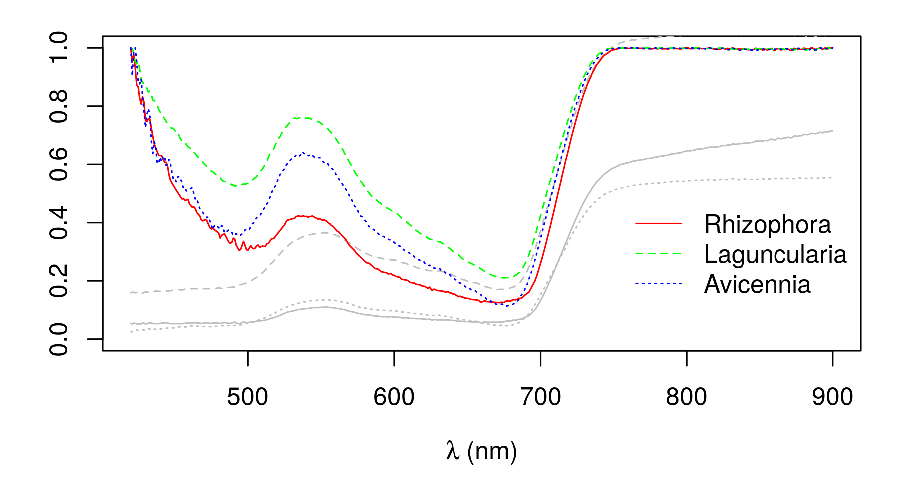
\includegraphics[width=\linewidth]{./Graficos/ContinuumR2.eps}
\end{frame}

\subsection{Combinaciones}
\begin{frame}{{\footnotesize 4-3-2}}
	\centering
	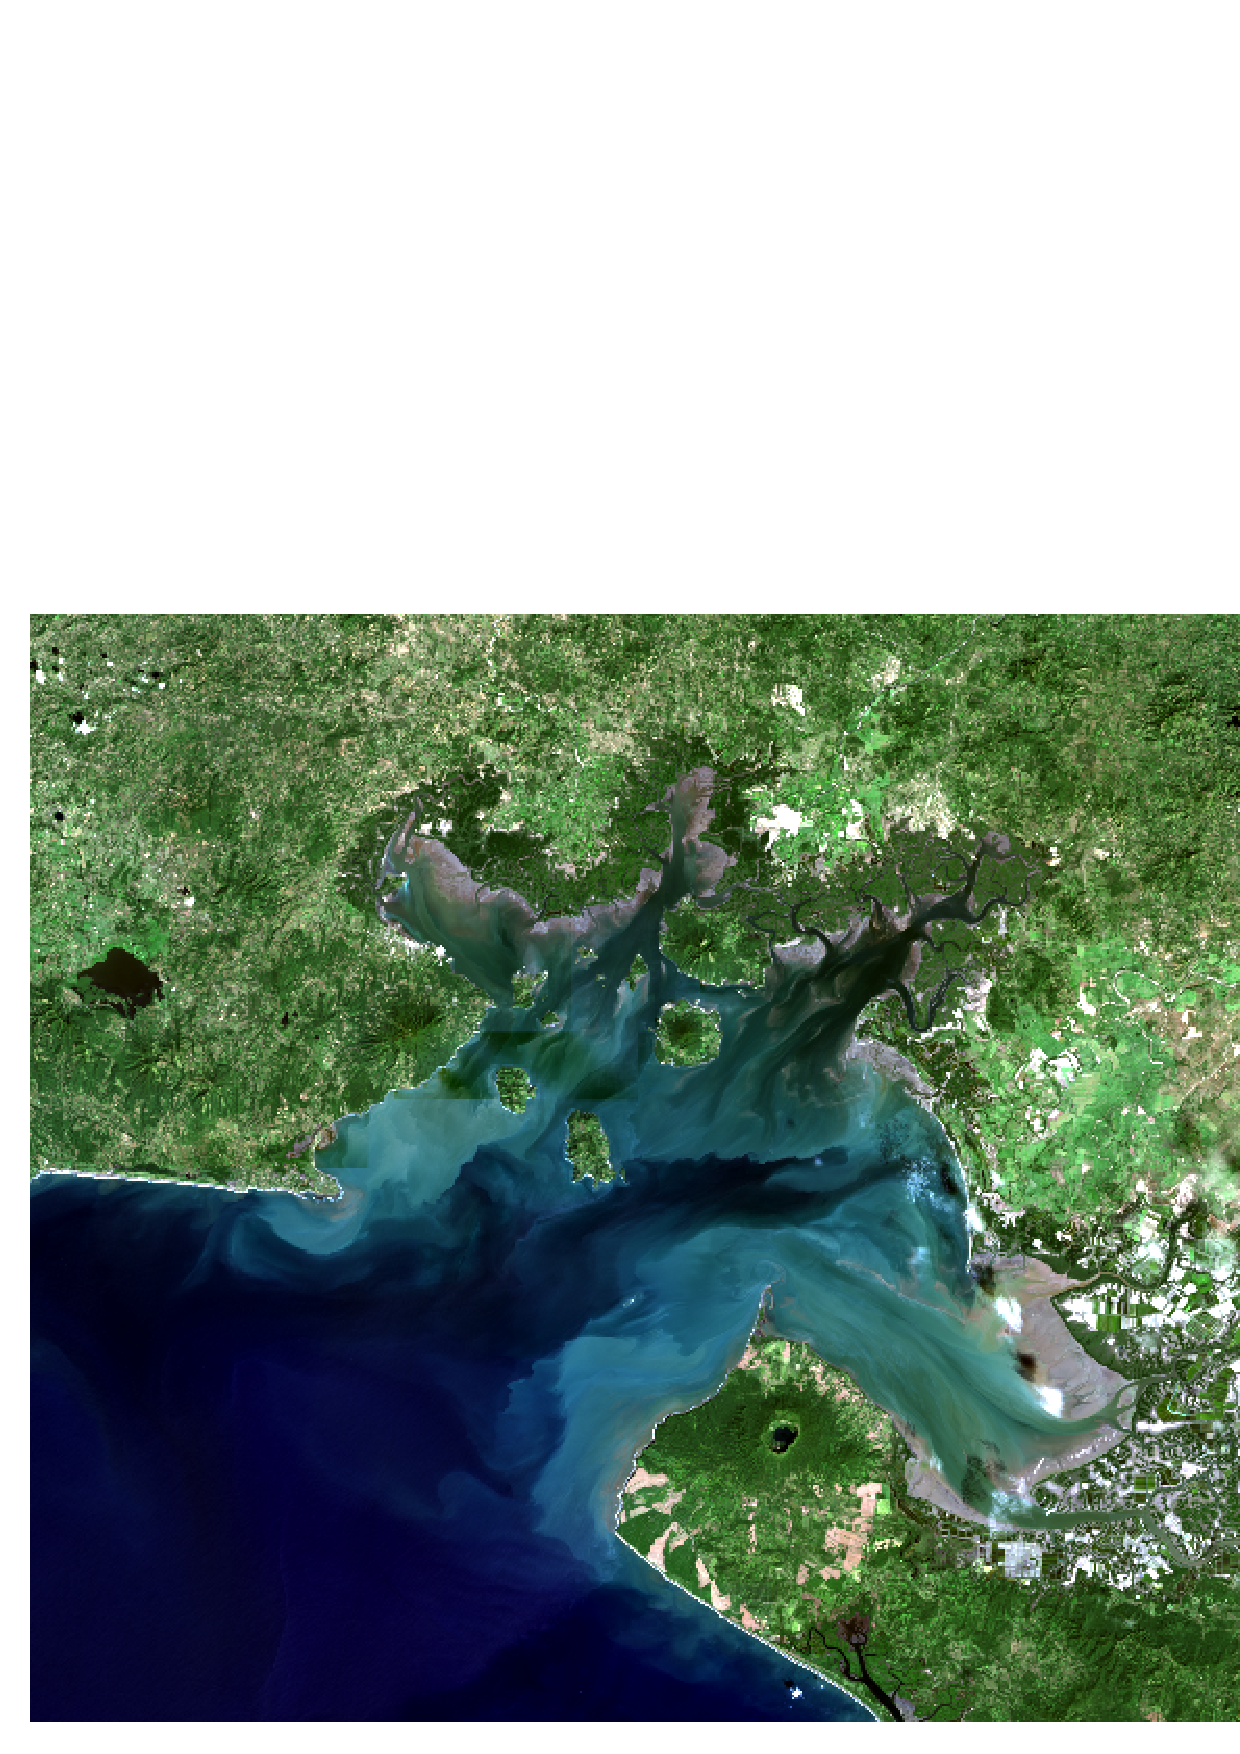
\includegraphics[width=0.8\linewidth]{./Imagenes/GF432.png}
\end{frame}

\begin{frame}{{\footnotesize 5-4-3}}
	\centering
	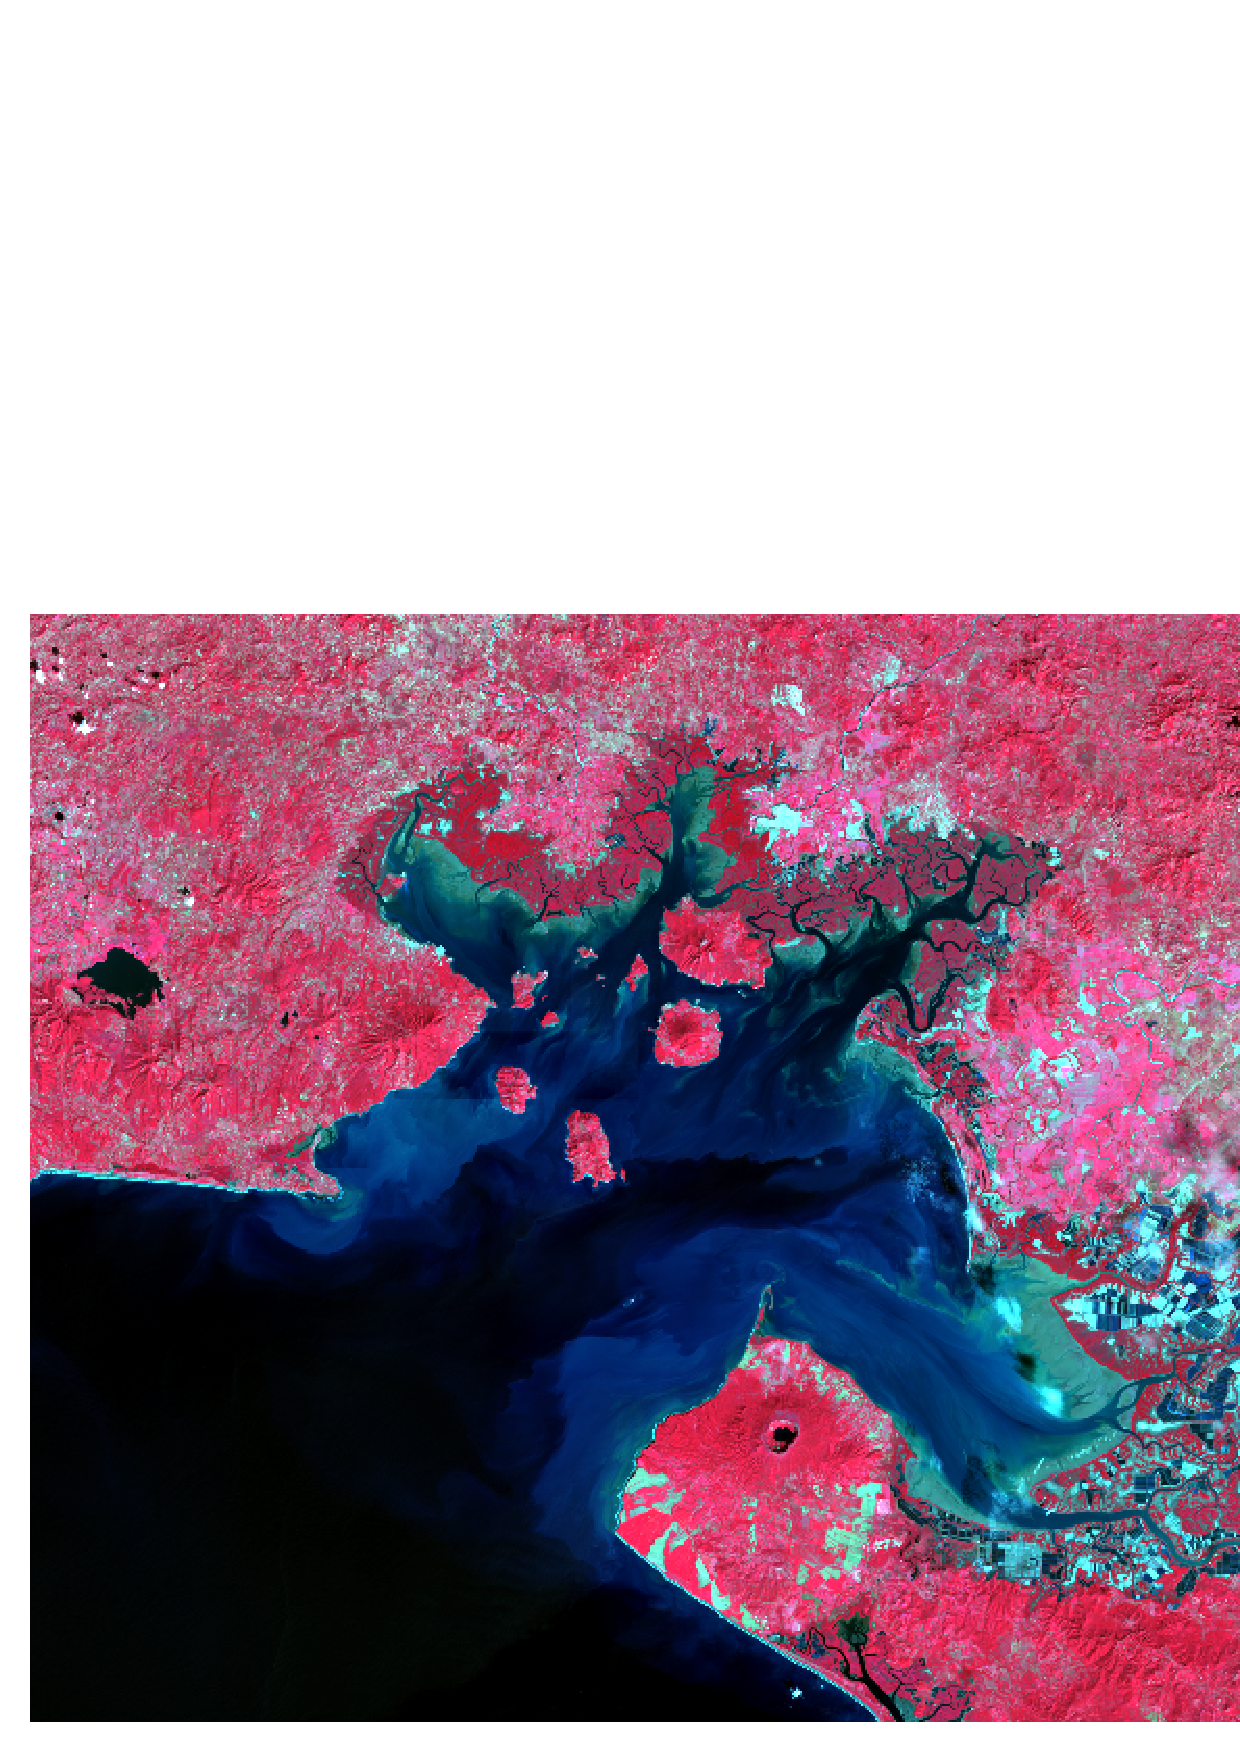
\includegraphics[width=0.8\linewidth]{./Imagenes/GF543.png}
\end{frame}

\begin{frame}{{\footnotesize 5-6-2}}
	\centering
	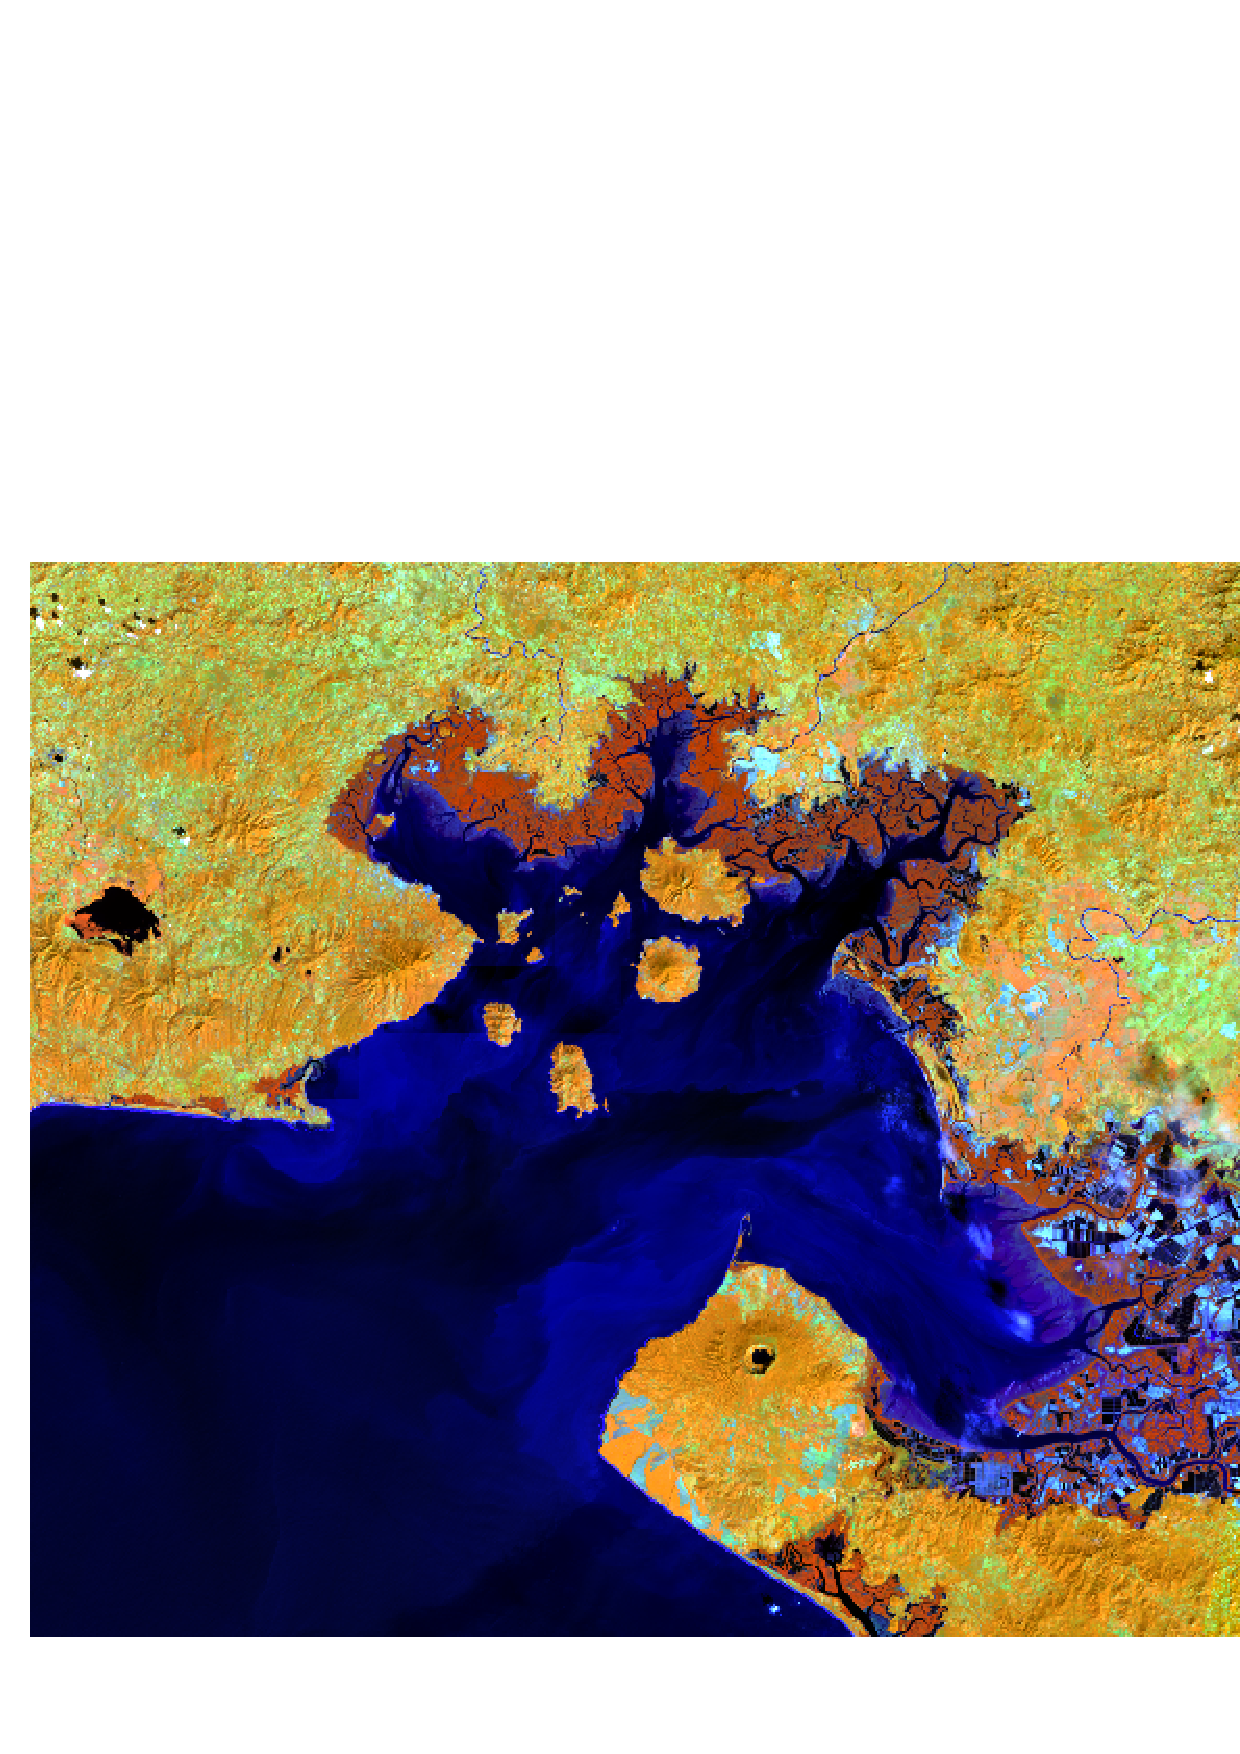
\includegraphics[width=0.8\linewidth]{./Imagenes/GF562.png}
\end{frame}

\begin{frame}{{\footnotesize 6-5-4}}
	\centering
	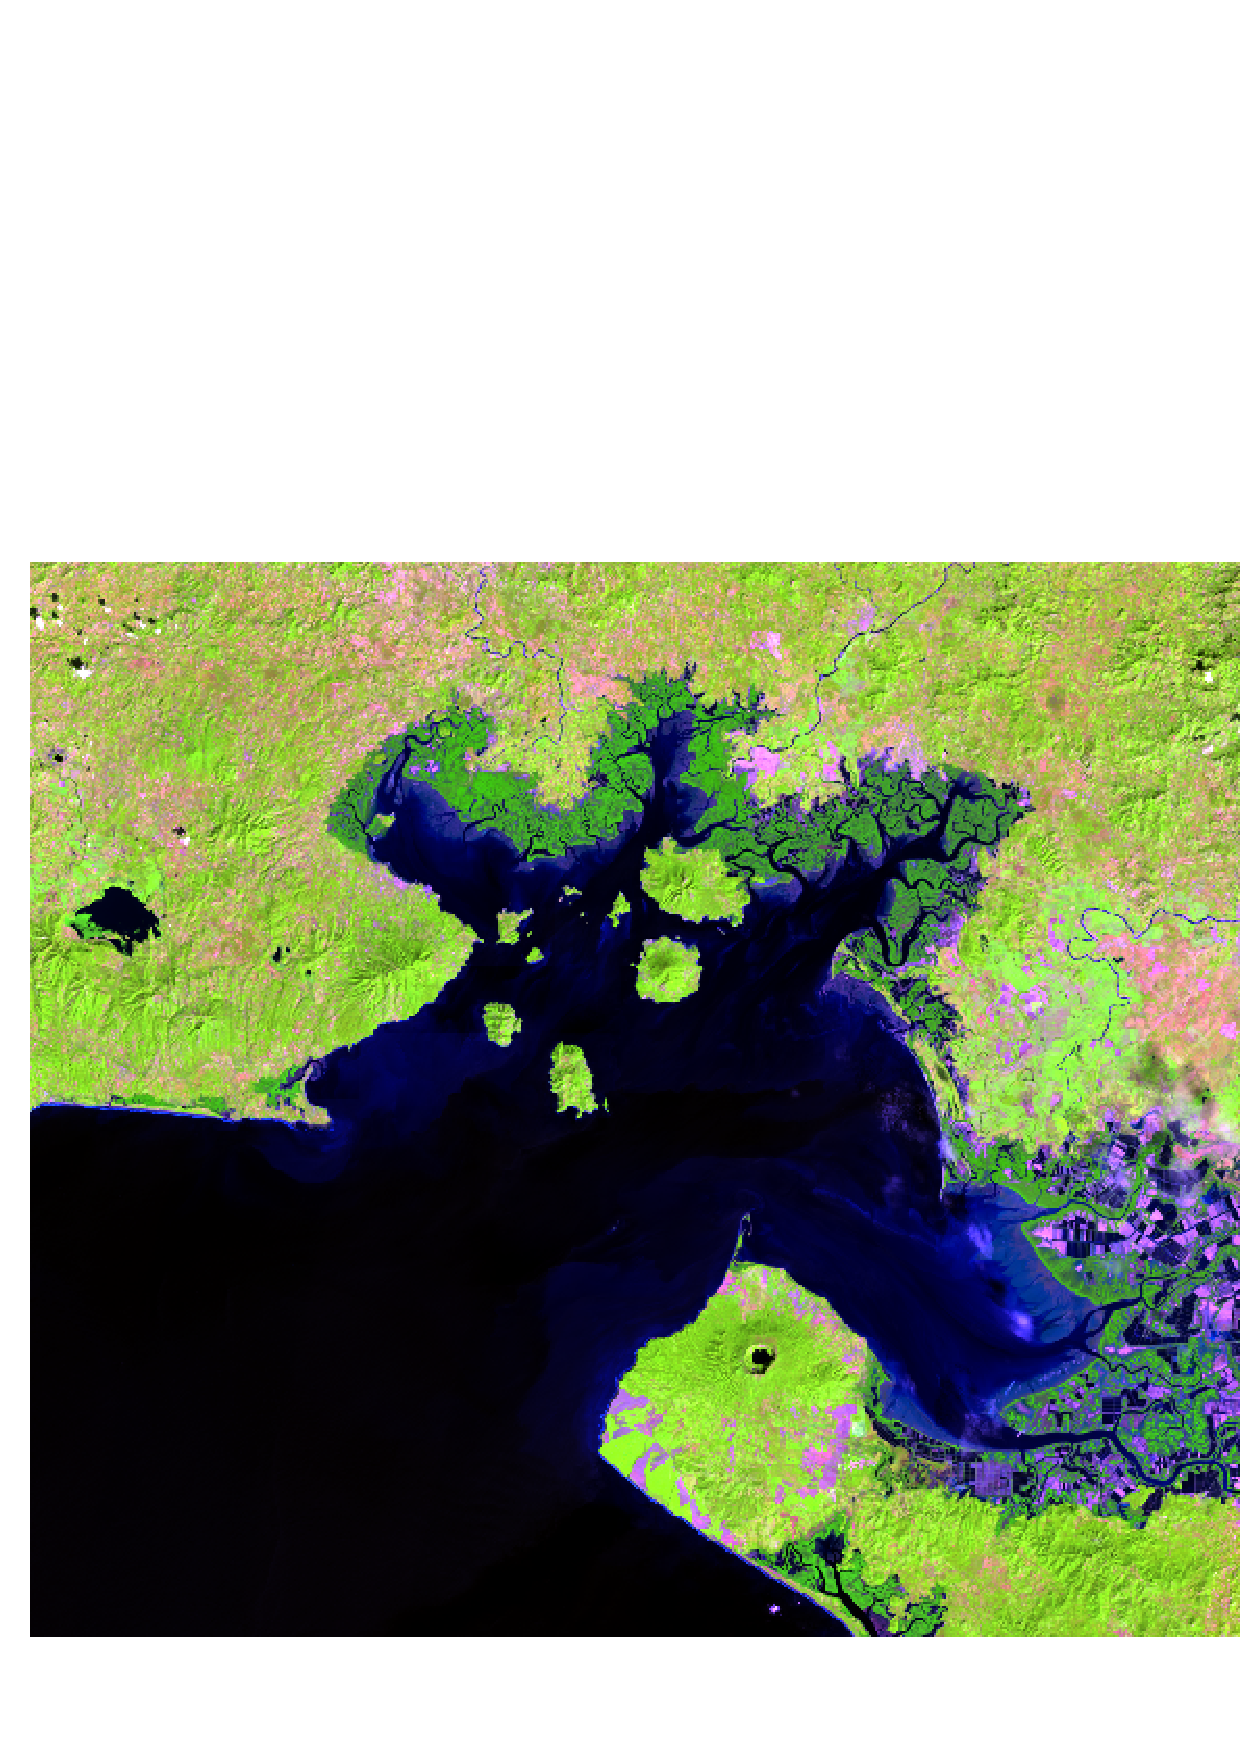
\includegraphics[width=0.8\linewidth]{./Imagenes/GF654.png}
\end{frame}

\subsection{Clasificación}
\begin{frame}{\footnotesize Clasificación no supervisada}
	\centering
	\includegraphics[width=0.8\linewidth]{./Imagenes/Classnosup.png}
\end{frame}

\begin{frame}{{\footnotesize Clasificación supervisada}}
	\centering
	\only<1>{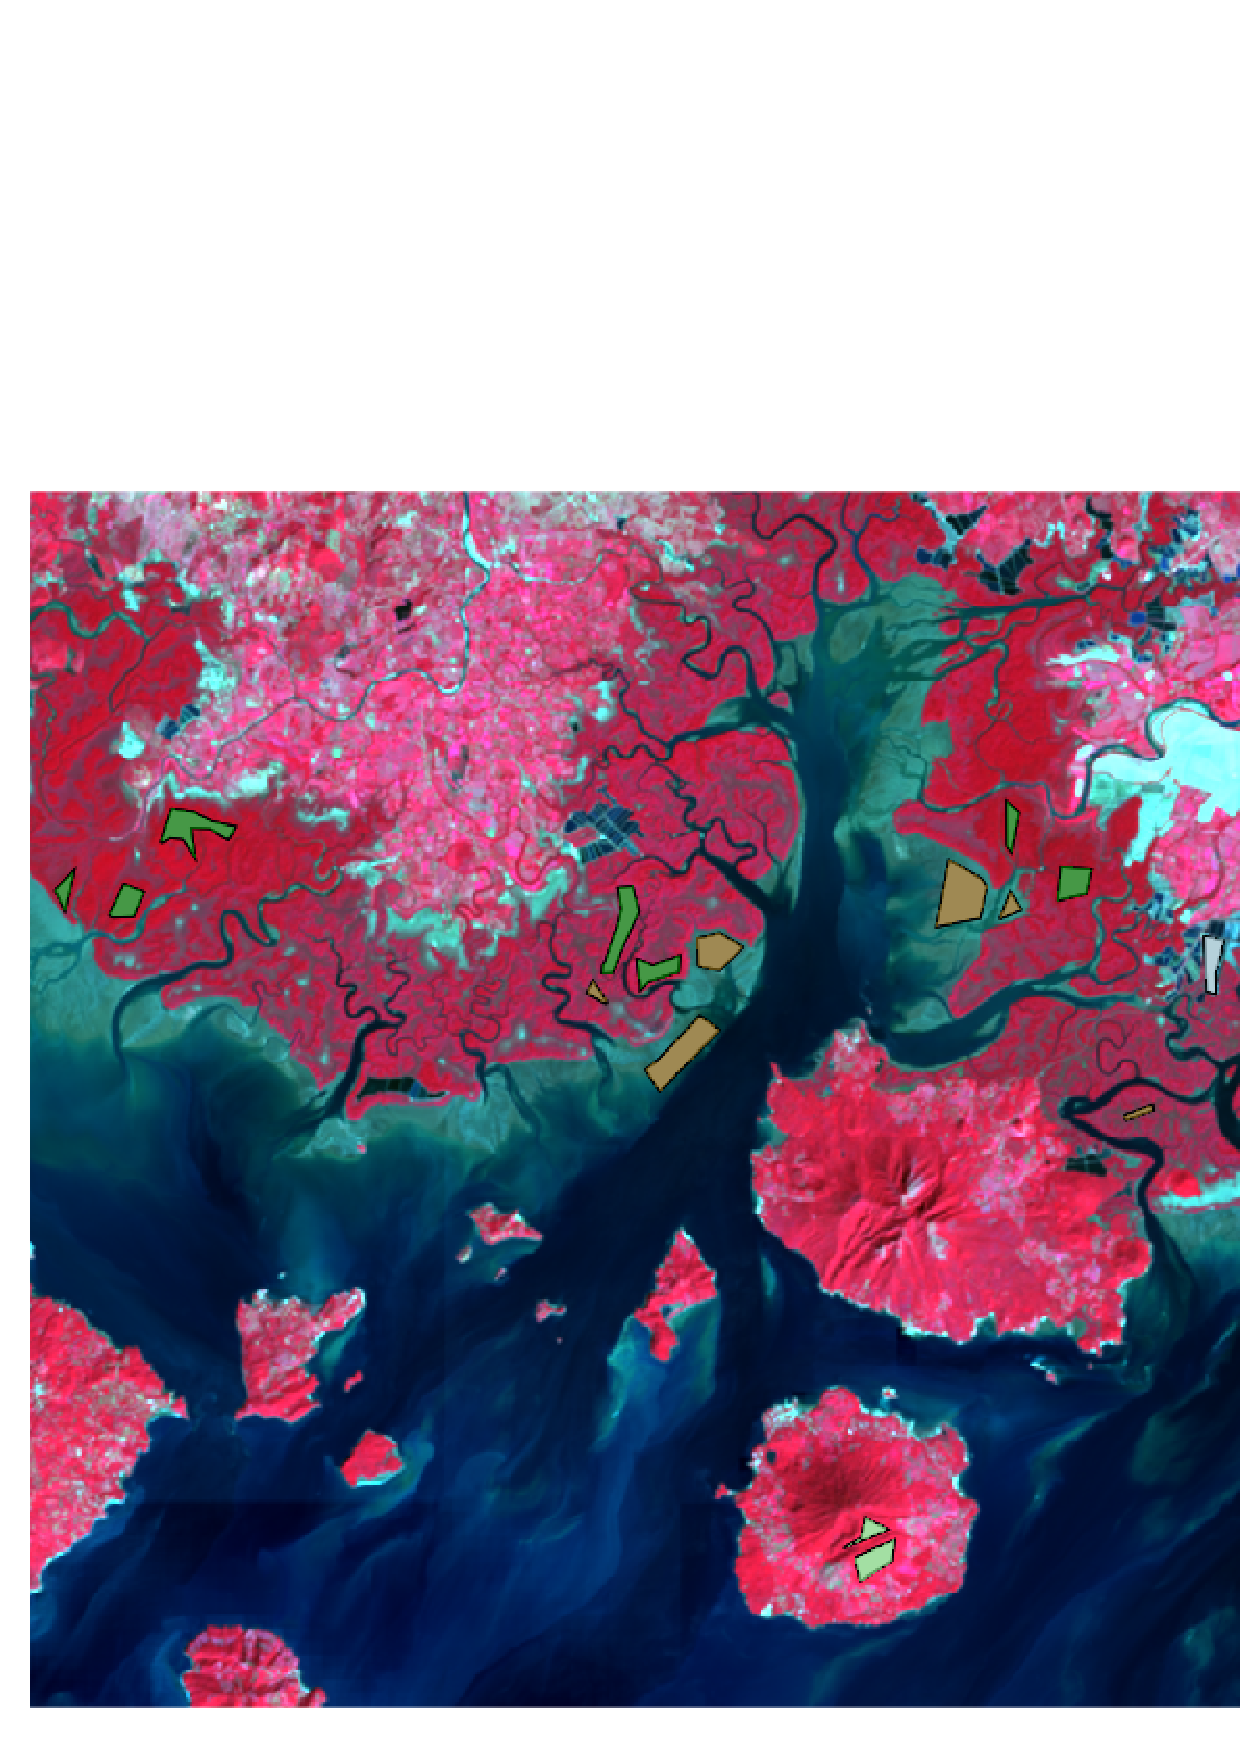
\includegraphics[width=0.6\linewidth]{./Imagenes/Detalle_training.png}}
	\only<2>{\includegraphics[width=0.8\linewidth]{./Imagenes/Classup.png}}
\end{frame}

\begin{frame}{{\footnotesize Spectral Angle Mapper}}
	\centering
	\includegraphics[width=0.8\linewidth]{./Imagenes/SAM.png}
\end{frame}

\subsection{Índices de Vegetación}
\begin{frame}{\footnotesize NDVI}
	\centering
	\includegraphics[width=0.8\linewidth]{./Imagenes/NDVI.png}
\end{frame}

\begin{frame}{\footnotesize SAVI}
	\centering
	\includegraphics[width=0.8\linewidth]{./Imagenes/SAVI.png}
\end{frame}

\section{Discusión y conclusiones}
\subsection{Discusión}
\begin{frame}
	\begin{block}{Aspectos a tener en cuenta}
		\begin{itemize}[<+->]
			\item Tomar más de una observación por especie
			\item Imágenes satélite con mayor resolución espacial y espectral
			\item Utilización del plugin SCP de QGIS
			\item Crear máscara o hacer un análisis de Componentes Principales
			\item Mejorar la toma de áreas de entrenamiento
		\end{itemize}
	\end{block}
\end{frame}

\subsection{Conclusiones}
\begin{frame}
	\begin{block}{Consideraciones finales}
		\begin{itemize}[<+->]
			\item Poca separabilidad entre \textit{R. mangle} y \textit{A. germinans}
			\item Mayor separabilidad de \textit{L. racemosa}, sobre todo con \textit{R. mangle}
			\item Resolución espacial de las imágenes Landsat 8 insuficiente
			\item Fácil detección del bosque de mangle, las salineras y los estanques
			\item Software libre útil y práctico en todas las fases del trabajo
		\end{itemize}
	\end{block}
\end{frame}

\appendix
\section{Recordatorio}
\begin{frame}
	\centering
	{\large \textbf{{\color{blue} \url{https://github.com/MarcosRial/TFG}}}}\\ \vspace*{2cm}
	Gracias por la atención
\end{frame}

\end{document}